\documentclass[9pt]{article}
\usepackage[utf8]{inputenc}
%\renewcommand{\baselinestretch}{1}
% Chagne the cite color 
\usepackage{geometry}
 \geometry{
 a4paper,
 total={170mm,257mm},
 left=20mm,
 top=20mm,
 }
\usepackage[table,xcdraw,svgnames]{xcolor}
\usepackage[colorlinks]{hyperref}
\AtBeginDocument{%
  \hypersetup{
    citecolor=Blue,
    linkcolor=Red,   
    urlcolor=Orchid}}

\usepackage{titling} % https://tex.stackexchange.com/questions/61919/set-position-for-maketitle-in-article
\newcommand{\subtitle}[1]{%
  \posttitle{%
    \par\end{center}
    \begin{center}\large#1\end{center}
    \vskip0.5em}%
}
\usepackage{graphicx}

% \title{ECE 752 Project Proposal}
\setlength{\droptitle}{-1cm}
\title{\textbf{Acc++: Accelerator for C++ STL}}
\subtitle{\textbf{phase 1 progress report}}
\author{\textit{Chen Chen, Yifan Hong, Yunhan Hu, Zirui Tao}}
\date{\today}

\begin{document}

\maketitle
\section{Introduction}
The phase 1 report consists of trails of profiling tools, profiling analysis on real applications, and proposed ideas for acceleration, which follows from the chronological order of project progress.

\section{Profiling tools} 
\subsection{GNU gprof} \label{sec:gprof}\\
% Cite: https://sourceware.org/binutils/docs/gprof/
The GNU profiler gprof \cite{graham1982gprof} uses a hybrid approach of compiler assisted instrumentation and sampling. To gather profiling information at runtime, the program counter is probed at regular intervals by interrupting the program with the operating system interrupts. Yifan first realized that as sampling is a statistical process, the resulting profiling data are not exact but are rather a statistical sampling approximation by gprof with induced bias. In addition, as we found that, it has been reported as sometimes losing track of parent function, as mentioned in \href{https://stackoverflow.com/questions/16664288/some-doubts-about-the-graph-generated-by-gprof-and-gprof2dot}{this discussion}. Nevertheless, since gprof is relatively stable and widely used, \textbf{we select it as the primary profiling analysis tool} in this project. Other than these two drawbacks, gprof provides a clean representation of the histograms of time spent on each function based on its total samples. This part is primarily done by Chen Chen. 

\subsection{gperftools} \label{sec:gperftools}\\
% Cite: https://github.com/gperftools/gperftools/wiki\\
Gperftools \cite{gperftools} from Google provides a set of tools aimed at analyzing and improving the performance of multi-threaded applications. We focus on their sampling-based CPU profiler, which has a very little runtime overhead, provides some nice features like selectively profiling certain areas of interest and has no problem with multi-threaded applications. Unfortunately, when we profile with gperftools, the profiler shows raw hex addresses instead of function names, which doesn't profile analysis friendly. This name mapping bug with x86-64 system is also reported by others and still not solved. Therefore we have to set it aside temporarily. This part is primarily done by Yifan Hong. 

\subsection{Pin}\\
The pin tool \cite{luk2005pin} is a software instrumentation tool by Intel that allows easy, programmable profiling tools. It provides a variety of profilings such as, all of which is is implemented through a C++ class API, which handy to customize. In this project, Zirui followed through the \href{https://www.dreamlandcoder.com/system-security/how-i-learned/intel_pin/}{DreamLandCoder's} blog on implementing instrumentation of program that outputs the accessed memory address and values, which is accessible to \href{https://github.com/tzrtzr000/AccPlusPlus/blob/master/pin/memTrace.cpp}{Project code repository}. This allows Pin to be a very powerful programming instrumentation tool to analyze almost any program behaviors. However, our goal is to analyze the performance bottleneck, the aforementioned \ref{sec:gprof} and \ref{sec:gperftools} are sufficient for estimating the time utilization for each leaf function.
This part is primarily done by Zirui Tao. 

\subsection{Valgrind}\\
Valgrind is a powerful software development tool that can be used to analyze memory errors, function calls, cache usage, stack and heap management, and multi-threaded contention. In this project, we use the callgrind, recording function calls and generating call graphs, and cachegrind, counting the cache misses and hits, in the Valgrind. The function of callgrind overlaps with the function of the previous tools, so it is only used to be a reference. Cachegrind is the main tool used. For the benchmarks we interest, we will record the cache usage. For the benchmarks with high hit rates, we will give up because they are hard to be improved. This part is primarily done by Yunhan Hu. 

% C++ is one of the most popular general-purpose programming languages due to its extension of C language with additional programming features such as object-oriented programming generic and functional features in addition to low-memory manipulation. Recently, there are ongoing research interests for building hardware-level optimization on popular software languages. Gope et al. \cite{gope2017architectural} examined the inexpensive hardware accelerator options for PHP applications via thorough profiling analysis. Meanwhile, there are emerging works that start looking into the hardware accelerator option on some specific C++ standard functions \cite{kanev2017mallacc}. After exploring the methodology of \cite{gope2017architectural} and report from \cite{kanev2017mallacc}, one natural question is to explore whether there exist opportunities to discover the overhead of existing C++ standard library (STL) and further optimize in hardware level. Thus, the goal of this project is to build the accelerator for C++ STL.

\section{Profiling Analysis}\label{sec:pa}

In total, we examined the gprof on matrix pseudoinverse operation using Arma, Opencv and Eigen separately, originally written by \href{http://nghiaho.com/?p=1726}{Nghia Ho}, which could be accessed through our \href{https://github.com/tzrtzr000/AccPlusPlus/benchmarks}{code repository} under benchmarks. In addition, we also examined \href{https://baptiste-wicht.com/posts/2017/05/cpp-containers-benchmark-vector-list-deque-plf-colony.html#fill}{\textit{Fill}} benchmark, provided by Wicht \cite{wicht_2017}. Due to the page limit, we instead focus on reporting the analysis case of the \textit{Fill} benchmark.

The \textit{Fill} benchmark analyzes the time complexity of STL C++ containers, such as vector, deque and list, upon invoking \textit{push\_back} leaf function. The size of testing elements ranges from 100,000 to 1,000,000. Table \ref{tab1} shows that over 80\% of system time is taken up by a GNU extension function to the Standard C++ Library, called \textit{new\_allocator}\cite{libstdc}, which uses \textit{global new} to manage heap memory allocation. 

After determining the leaf function with the highest contribution, we begin to analyze its underlying mechanism. To isolate the analysis of \textit{push\_back} function, we write a simple program that contains \textit{std::vector} with \textit{push\_back} function and compiled C++ source code to x86 based assembly instructions. We then manually traced the program order using \textit{gdb} and discovered that the \textit{new\_allocator} handles the allocation and de-allocation operation of std::vector's elements, according to \cite{libstdc}. Additonally, we used gprof and grof2dot to convert profiling output to function calls as directed acyclic graphs(DAG), as shown in Fig. \ref{fig:func_dag}.

The \textit{Fill} benchmark helps us get familiar with couple analysis tools. We then proceed similar analysis on a real applicaton: matrix pseudoinverse operation benchmark, with Arma, Openvv and Eigen environments separately. By profiling real benchmarks, we discovered some accelerators design opportunities which is covered in section \ref{sec:pp}.

\begin{table}[htbp]
\begin{center}
\begin{tabular}{|c|c|}
\hline
 \textbf{Leaf Function}&\textbf{Time Contribution \%}\\
% \cline{2-4} 
\hline
new\_allocator(Trivial(4096)) & 64.49\\
\hline
new\_allocator(Trivial(1024)) & 16.37\\
\hline
new\_allocator(std::list(4096)) & 2.80\\
\hline
new\_allocator(Trivial(128))   & 1.35\\
\hline
other                          & 14.99\\
\hline
\end{tabular}
\caption{Leaf Function Contribution, table generated by Chen Chen}
\label{tab1}
\end{center}
\end{table}

\begin{figure}[t]
    \centering
    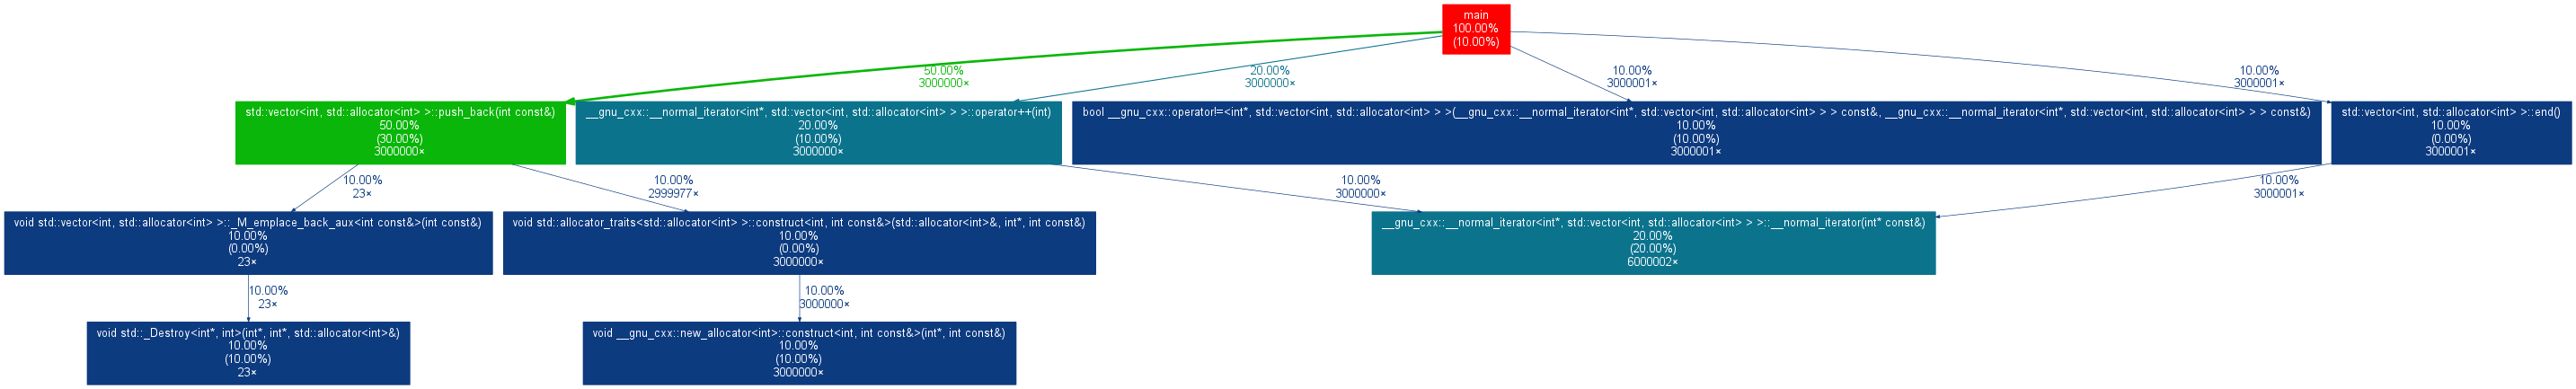
\includegraphics[width=12cm,  height=9cm,
    keepaspectratio]{figures/func_dag_t.png}
    \caption{function DAG for simple \textit{push\_back} to \textit{std::vector} program, cutoff at 10\% runtime for visualization, figure generated by Zirui. Full figure can be access through: \url{https://github.com/tzrtzr000/AccPlusPlus/blob/master/ref/func_dag_t.png}}
    \label{fig:func_dag}
\end{figure}

% Wicht \cite{wicht_2017} analyzed the run time of C++ containers with the most commonly used functions: Insertion, Iteration, Search, Sort, etc., by varying the number of elements and the type of data. It showed that \textit{list} had the slowest iteration but fast insertion. While \textit{deque} had good iteration but slow insertion. The weakness of each container implied chances to mitigate them by implementing specialized accelerators.\\



\section{Proposed Plan}\label{sec:pp}
Based on the analysis on all applications mentioned at the beginning of \ref{sec:pa}, not limited to one reported, we proposed three potential ideas for accelerating C++ programs.  


\subsection{Memory Allocation}\\

By tracing through assembly through gdb, we found that "insert" operation (\textit{push\_back, Fill}) generates a great number of instructions (~s200) to only allocate new heap memory space, which shows opportunities to design accelerators for dynamic memory allocation and size of class computation. 

Although existing literature \cite{kanev2017mallacc} has examined the solutions on accelerating malloc function specifically on C++, it is still possible for us to find alternative design strategy for heap manager. Intuitively, the heap management process should take up a critical portion of computation time in real applications, which still worth us to understand it deeply.

\subsection{Iterator Implementation}\\

As a significant part in C++ STL, iterators are primarily used in sequence of numbers, characters etc. As shown in Fig.\ref{fig:func_dag}, for instance, iterator functions are the second most overhead after allocation. In some particular simple benchmark the percentage of iterators can even reach 60\%. Therefore, finding optimization opportunities on hardware-level for iterators would be promising and worth trying. Next step we will dive in iterators' instruction-level behaviors, trying to achieve some regular patterns, then optimize the implementation for specific usage.

% The basic assumption of designing an accelerator is that certain instructions can be run on customized hardware extra hardware units instead of the normal architecture for higher resource utilization. In fact, there exist hardware accelerators for varying computing demands (such as GPU for graphics computing and TPU for AI-related computation). Our idea is to analyze C++ benchmarks and find out the high-frequency functions and potential overhead bottlenecks. Then, we will choose several activities for optimization, analyze its running path and operational characteristics of the instruction, find out redundant parts, and design a special operating unit for it.\\

\subsection{Value Assignment Speculation}\\
After the analysis, Chen noticed that the \textit{push\_back} function copies the value of the source variable and moves it into the vector container, which requires expensive copy instructions and the system may need to spend extra time to remove the reference\cite{cplusplus.com} from source variables. A novel value assignment speculation scenario can be designed to release this pressure.

In C++ syntax, there exists a fundamental implementation difference between Lvalue and Rvalue assignment: move or copy values from the source to the destination. \cite{rvalue_intro, rvalue_ref}. In short, Lvalues' assignments maintain source values while Rvalues' assignment does not, which involves the expensive copy instructions and cheap moving pointer operation separately. While newly introduced C++ compiler specifically distinguishes the Lvalues and the Rvalues through rigid static definition, Zirui proposed that during dynamic execution, some Lvalue reference could be equivalent to Rvalue reference (as long as there is no write to either source and destination variable). By presenting a subset of Lvalue as Rvalue, the execution would be able to benefit from extra performance gain from Rvalue implementation. As discussed with Prof. Lipasti, OS already adopted the Copy on Write (COW) \cite{wiki:Copy-on-write} policy, in which a copy from the instruction of duplication is deferred until writes: the source and destination would initially share the same physical address. An OS exception occurs when either one of the variables performs a write operation, in which a memory allocation is performed, followed by a value calculation and assignment. The COW policy is based on the assumption that all assigned operators tend not to be written as frequent as to be read, thus, avoiding copes in the first place could benefit from the performance and memory allocation, even the penalty for extra OS exception handling for write is expensive. Similar to branch prediction and value prediction, Zirui proposed that there may be opportunities for the predictor to predict read and write pattern for certain variables. However, in order to maintain the correctness of execution, the source value should still be efficiently "tracked", therefore a follow-up solution is to design a data buffer for hardware to handle write exception normally handled by OS. The plan for this idea is to first examine whether this idea would have a significant impact on performance or energy efficiency. If it does, then a follow up fine-grained experiments would be performed to exploit the most ideal design parameter. 

% First, we will start with running several C++/STL benchmarks, analyze the code and performance to find the distribution of CPU cycles of functions in order to select several major overheads to optimize.  Note that Wicht \cite{wicht_2017} provided a nice container analysis in his \href{https://baptiste-wicht.com/posts/2017/05/cpp-containers-benchmark-vector-list-deque-plf-colony.html}{blog}, so by identifying the utilization rates ($<\textit{container types}>, <\textit{function}>$) pairs, we then would (hopefully) be able to observe the most frequent performance/resource bottleneck.\\
% Then we will perform hardware acceleration to those activities, design our accelerating units based on functions’ behaviors. Our design will be simulated on gem5 to evaluate performance comparing to the original situation. This part will be mainly programmed in C++.\\
% Finally, if time permits, we will dive into the hardware level, attempt to implement our accelerator in Verilog, synthesize it to evaluate the area, power, delay, etc.\\


{
\bibliographystyle{IEEEbib}
\bibliography{ref}
}
\end{document}